\section{Generative Adversarial Networks}
\begin{figure}
	\centering
	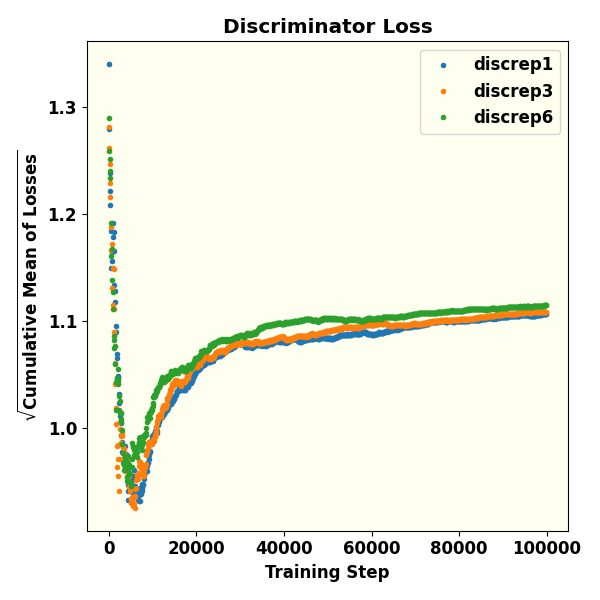
\includegraphics[width=\linewidth]{fig/analysis/Discrep_Runs_Losses_disc_loss.png}
	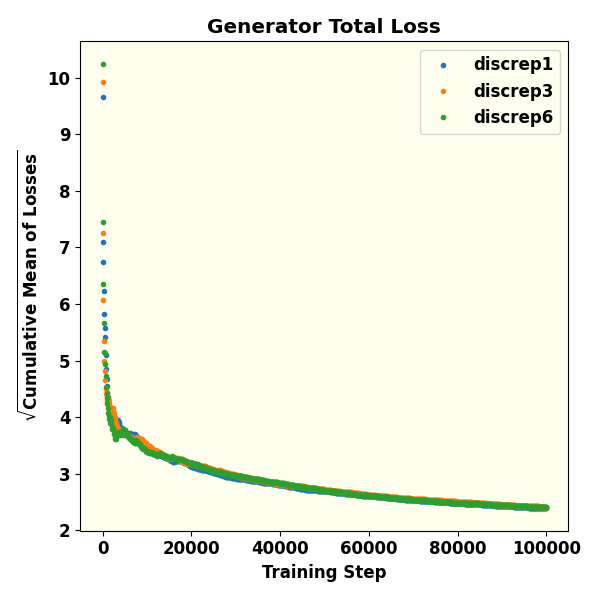
\includegraphics[width=\linewidth]{fig/analysis/Discrep_Runs_Losses_gen_total_loss.png}
	\caption{The number of episodes of Discriminator training per every episode of Generator training (termed Discriminator repetition or Disc. rep.), understandably, has a higher impact on the Discriminator loss than on the Generator loss. The left	and the right panel show this effect on the square root of cumulative mean of Discriminator loss and the Generator loss respectively.}
	\label{fig:Plot_discrep_loss}
\end{figure}
\begin{figure}
	\centering
	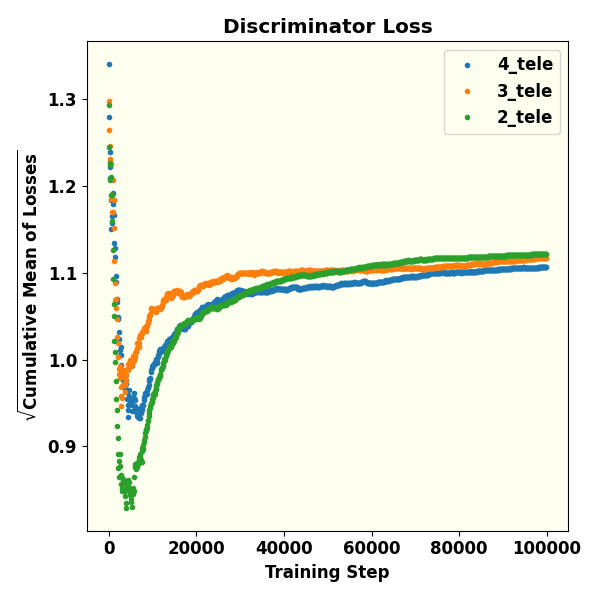
\includegraphics[width=\linewidth]{fig/analysis/Telescope_Runs_Losses_disc_loss.png}
	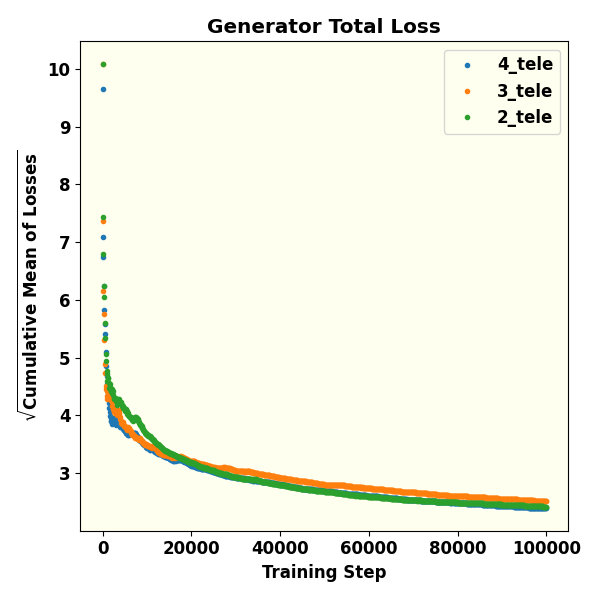
\includegraphics[width=\linewidth]{fig/analysis/Telescope_Runs_Losses_gen_total_loss.png}
	\caption{The square root of cumulative mean of Discriminator and Generator loss for different numbers of telescopes. It has a very significant impact on the model performance. If there are only two telescopes, both Discriminator and Generator are not trained smoothly. The result of four telescopes is a lot better because the cumulative mean of loss functions is smaller compare to other parameters.}
	\label{fig:Plot_telescopes_loss}
\end{figure}
Generative Adversarial Networks (GANs) were introduced by \cite{goodfellow2014generative}. The underlying concept is straightforward: it involves two competing networks. The first network, known as the Generator, produces new images based on an input image. These will be referred to as generated images. The second network, the Discriminator, attempts to distinguish between the generated image (predicted image) and the real image (ground truth) using Discriminator loss function.

Through the alternating training of these networks, the generated images gradually become indistinguishable from the real images. Essentially, this process constitutes a two-player min-max game --- a classic problem in game theory. The original formulation of GANs is given by:
\begin{equation}
	\centering
	\begin{aligned}
		\min_{G} \max_{D} V(D, G) &= \mathbb{E}_{x \sim p_{\rm data}(x)} \left[ \log D(x) \right] \\
		&+ \mathbb{E}_{z \sim p_{z}(z)} \left[ \log \left( 1-D(G(z)) \right) \right]
	\end{aligned}
	\label{eq:Basic_GAN}
\end{equation}
where $V(D, G)$ denotes the value function of the min-max game.

The objective is to learn the Generator's distribution, \(p_G\), over the data \(x\). We begin with input noise variables \(p_z(z)\) and employ two perceptrons, \(G(z; \theta_G)\) and \(D(x; \theta_D)\), parameterized by \(\theta_i\) with \(i = G \ \mathrm{or}\ D\) respectively. Here, \(G(z)\) is a differentiable function that maps \(z\) to the data space \(x\), while \(D(x)\) represents the probability that \(x\) originates from real data. The problem can be reformulated as:
\begin{equation}
	\centering
	\begin{aligned}
		\max_{D} V(G, D) &= \mathbb{E}_{x \sim p_{\rm data}} \left[ \log D^{*}_{G}(x) \right] \\ 
		&+ \mathbb{E}_{x \sim p_{G}} \left[ \log \left( 1 - D^{*}_{G}(x) \right) \right]
	\end{aligned}
	\label{eq:GAN_reformulated}
\end{equation}
where \(D^{*}_{G}\) denotes the optimum of the discriminator for a given fixed generator, as shown in equation (\ref{eq:Disc_optimum}). It can be demonstrated that the global optimum of equation (\ref{eq:GAN_reformulated}) is achieved if and only if \(p_G = p_{\rm data}\). Furthermore, if both \(G\) and \(D\) are allowed to reach their respective optima, then \(p_G\) converges to \(p_{\rm data}\). A more comprehensive discussion of the problem, including proofs, is provided in \cite{goodfellow2014generative}.
\begin{equation}
	\centering
	D^*_G(x) = \frac{p_{\rm data}(x)}{p_{\rm data}(x) + p_G(g)}
	\label{eq:Disc_optimum}
\end{equation}

Subsequently, the GAN framework was extended to a conditional model \citep{mirza2014conditional}. In this formulation, both the Generator and the Discriminator receive additional information $y$, and the value function of the conditional GAN (cGAN) is expressed as:
\begin{equation}
	\centering
	\begin{aligned}
		V(D, G) &= \mathbb{E}_{x \sim p_{\rm data}(x)} \left[ \log D(x|y) \right] \\
		&+ \mathbb{E}_{z \sim p_{z}(z)} \left[ \log \left( 1-D(G(z|y) \right) \right]
	\end{aligned}
	\label{eq:conditional_GAN}
\end{equation}
\cite{isola2017image} further observed that combining the cGAN from Eq.~\eqref{eq:conditional_GAN} with the traditional L1 loss improves the results, as the Generator is encouraged to produce outputs closer to the ground truth. Hence, the function that is minimized is:
\begin{equation}
	\centering
	L_{tot} = \arg \min_{G} \max_{D} V(D, G) + \lambda \cdot L_1(G)
	\label{eq:total_gen_loss}
\end{equation}
with the choice $\lambda = 100$ and
\begin{equation}
	\centering
	L_1(G) = \mathbb{E}_{x,y,z} \left[ ||{y - G(x,z)}||_1 \right]
	\label{eq:l1_loss}
\end{equation}
This type of network has demonstrated remarkable robustness across a variety of applications. For example, it can generate colored images from grayscale inputs based on architectural labels, transform images from day to night, and even predict maps from satellite data. A more extensive list of applications is provided in \cite{isola2017image}.


\subsection{Generator}
As discussed above, in a GAN the Generator is responsible for producing synthetic data—in this case, images that resemble those of a fast-rotating star. In this work, the Generator is implemented as a U-Net convolutional network \citep{ronneberger2015u}. In such architectures, the image's spatial resolution is first reduced through downsampling and then restored via upsampling, resulting in a U-shaped structure. The downsampling process typically involves convolutional layers followed by a strided operation (with a stride of 2) to effectively subsample the image, and a leaky version of the Rectified Linear Unit (LeakyReLU) is employed as the activation function.

In contrast, the upsampling process uses only the standard Rectified Linear Unit (ReLU) for neuron activation. This stage also comprises convolutional layers followed by operations with a stride of 2 to upscale the image to a higher resolution. Additionally, a dropout layer is introduced at the beginning of the upsampling phase to mitigate overfitting of the Generator model \citep{isola2017image}.

After generating images, the Generator aims to deceive the Discriminator into classifying the generated images as real. The extent to which the Generator succeeds in this deception is quantified by the GAN loss. When the Discriminator is unable to distinguish between the generated and real images (i.e., when the GAN loss is minimized), the Generator is considered to have reached an optimal state. Conversely, if the generated image fails to fool the Discriminator, the Generator produces a new image for further comparison with the real image. Additionally, the Generator's performance is evaluated using another metric known as the L1 loss, which is defined as the mean absolute error between the pixels of the real image and those of the generated image. Balancing the minimization of both the GAN loss and the L1 loss enables the Generator to produce images that are not only realistic but also faithful to the input data. 

\subsection{Discriminator}
The Discriminator is tasked with classifying the images produced by the Generator as either real or fake. It takes a real image from the dataset (often referred to as the target image for the Generator) and provides feedback to guide the Generator toward producing more accurate images. In this work, the PatchGAN model \citep{isola2017image} is employed as the Discriminator. Unlike a traditional global classifier, PatchGAN evaluates individual patches of the image, outputting a grid of predictions rather than a single scalar value.

The Discriminator’s architecture begins with an initializer that accepts both the input (generated) images and the corresponding real images. Initially, Salt-and-Pepper noise is added to the input images. PatchGAN then reduces the spatial dimensions of the images to extract localized features, ensuring the model focuses on smaller regions. In this downsampling stage, a leaky version of the Rectified Linear Unit (LeakyReLU) is applied in the convolutional layers, similar to the approach used in the Generator.

Subsequently, zero padding is applied, adding rows and columns of zeros around the images to prevent the loss of spatial information during convolution and to facilitate the extraction of deeper features from the downsampled output. Following this, batch normalization is employed to stabilize learning by normalizing activations, and the Discriminator begins classifying each patch as real or fake. This is followed by additional layers involving LeakyReLU activation, zero padding, and convolution, culminating in a final prediction that the Generator uses as feedback.

The effectiveness of the Discriminator is measured by its ability to distinguish between real and fake images, quantified through the Discriminator loss. This loss is composed of two parts: one that measures how accurately the Discriminator identifies real images (by comparing predictions to a target value of 1) and another that assesses how accurately it identifies fake images (by comparing predictions to a target value of 0). Together, these loss components ensure that the Discriminator improves its classification performance, which in turn challenges the Generator to produce increasingly realistic images.
